\chapter{Introduction}
\label{cha:intro}
\section{Importance of topic}
"Society expects autonomous vehicles to be held to a higher standard than human drivers." \cite{Prof.Amnon} This quote is setting the tone of the technology in autonomous driving. In order to be accepted to the public, autonomous vehicles should perform as least as good as the conventional human driver on parameters as for example safety. Despite widespread research on self-driving vehicles the acceptance by the user stays only limited.\cite{Bae2019} Out of investigation it followed that purchase behaviour of customers can be directly linked with comfort. Also in order to gain more trust by the public it is clear that the challenge of making autonomous vehicles as comfortable as possible, should be tackled. This immediately leads to the questions: what is exactly comfort during driving and how can it be measured?\\
Driving comfort is a personal experience and also depends on the current emotional state of the driver. This means that more than one driving style for autonomous vehicle-driving should be identified for a certain vehicle. \cite{Eindhoven2019} The state of the driver can be communicated with the vehicle at the start of each ride and different driving styles can be obtained by changing the parameters in a path planning algorithm. 

\begin{figure}[h!]
	\centering
	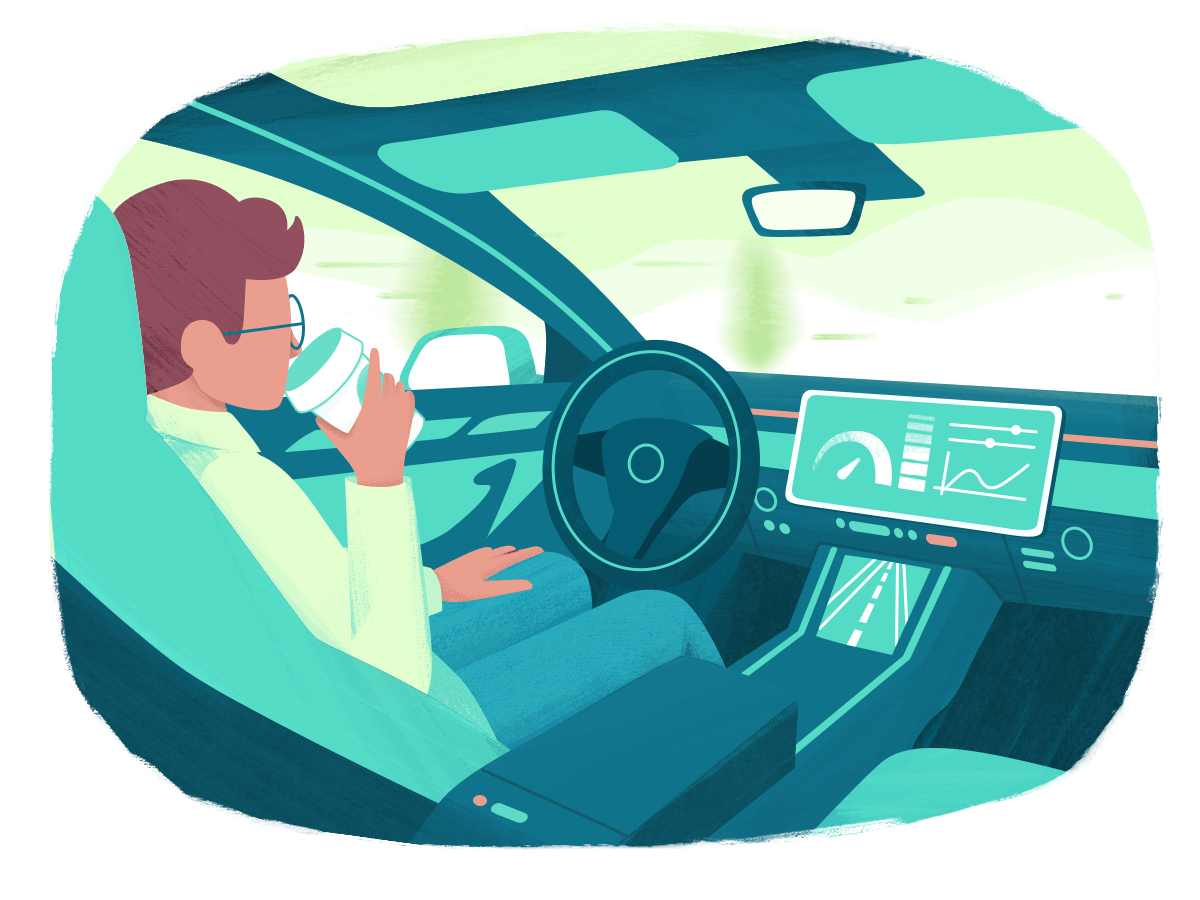
\includegraphics[width=0.50\linewidth]{AV}
	\caption{Concept visualization of autonomous driving. (source: \cite{AV})}
	\label{fig:AV}
\end{figure} 
\newpage

\section{Problem formulation and link with previous studies}
In order to identify specific comfort preferences of the driver that are quantized by parameters, the vehicle should be able to learn by demonstration. \cite{Kuderer2015a}\\
Despite that each driver has its own preferences, they are based on a common notion of comfort where different trade-offs are made. For example, some drivers prefer more aggressive driving than others, which will be manifested in a different set of parameters then which will be attained for a defensive driver for the same comfort criteria. The comfort criteria will later in this thesis be translated into an objective function where different weights are used in order to quantify different comfort trade-offs made. This approach is in literature called inverse optimal control or inverse reinforcement learning because it is learning the objective function for an optimal control problem.\\

In order to learn the weights which can be used to distinguish different drivers, research about the common notion of comfort is necessary. Passenger surveys in public road transport about carsickness \cite{Turner1999} have identified lateral acceleration as the primarily responsible for motion sickness. It is explained that drive style is a main factor to influence the amount of sickness and it was found that sickness is higher when drivers drove with a higher average magnitude of fore-and-aft and lateral motion. These effect were far more significant than the effect of vertical vibrations. There is also a consensus reached about the contribution of continuous trajectories to the prevention of motion sickness and the natural feel of paths.\cite{Elbanhawi2015} This means that higher order kinematic variables like accelerations and jerks also should be considered when measuring comfort. Chapter \ref{cha:Literature_study} will give a more detailed description on the literature study conducted in order to investigate the state of the art comfort modelling. Here will also the theory behind inverse reinforcement learning be discussed.\\

\section{Thesis objective and structure}
The goal of this thesis is to build further on the research of learning by demonstration conducted in \cite{Kuderer2015a} and to refine this idea by making use of more realistic vehicle models. Concretely the thesis is focussed on the implementation and validation of an algorithm that learns weights in a comfort objective function which can explain observed driver data.\\
The learning process is done offline. After the different weights are identified, the learned objective can be used to plan paths which can be followed by an autonomous vehicle, making use of an online tracking MPC.\\

To conduct the inverse learning control there is looked at data generated by simulations where it is assumed that the vehicle is driving on an straight road on high way speed. The maneuver investigated is a lane change maneuver as can be seen in Figure \ref{fig:lane_change}. In order to generate data, the non-linear bicycle and a more realistic $15$ dof of freedom Amesim model is used.\\

\begin{figure}[htp]
	\centering
	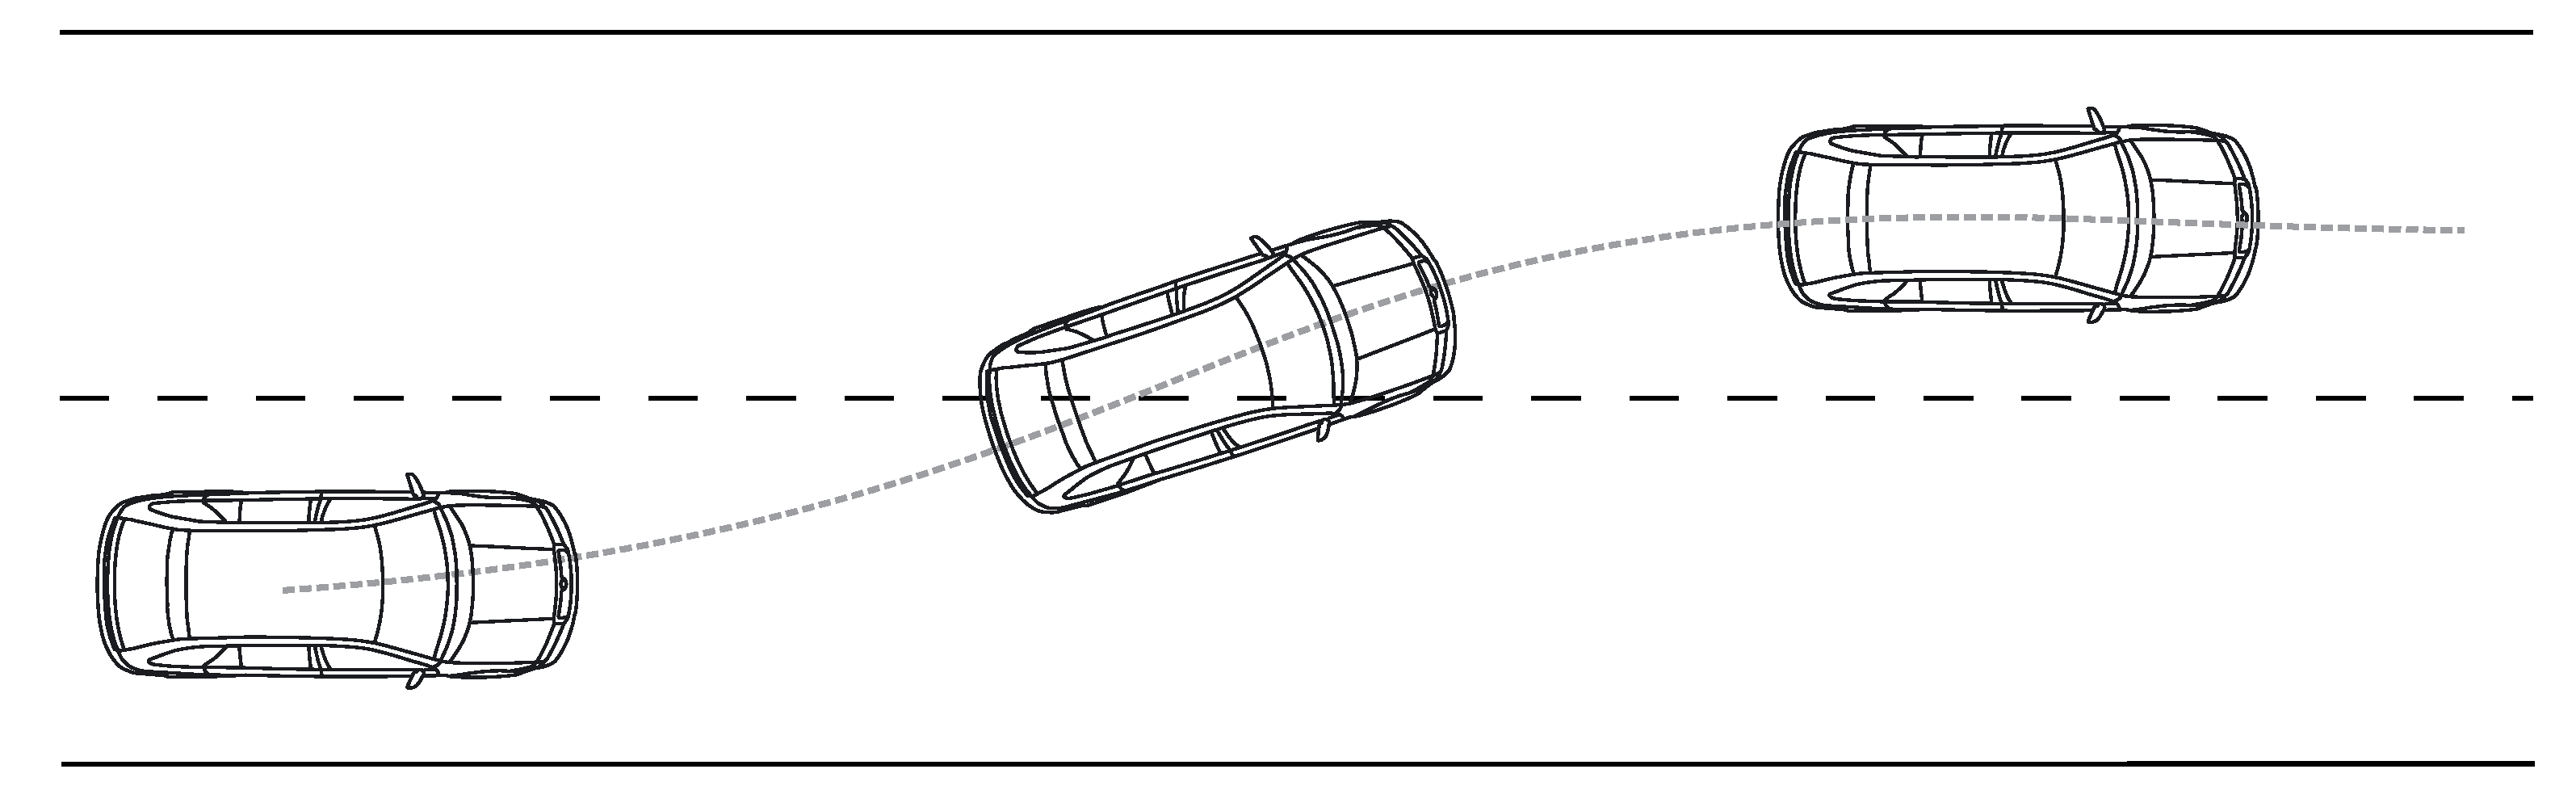
\includegraphics[width=0.8\textwidth]{lane_change.PNG}
	\caption{Example of a lane change which is the investigated maneuver in this thesis.}
	\label{fig:lane_change}
\end{figure}

The execution of this research is conducted with the support of "Siemens Digital Industries Software" located in Leuven which made it possible to preserve a direct link with reality. Software was made available i.d. Simcenter Amesim.\\

The structure of the thesis is build up as follows. First the reader is made acquainted with optimal control concepts that will be used in chapter \ref{cha:OCP}. In chapter \ref{cha:Literature_study} the state of the art of comfort modelling is discussed. This is split up in two parts. First the question what comfort during driving means, will be answered in section \ref{s:comfort_parameters}. The second part concerns a discussion on the inverse reinforcement learning concept used in section \ref{s:inverse re le}. Chapter \ref{cha:Learning_algorithm} gives insight in learning from ideal data. The non-linear bicycle model used is discussed in section \ref{sec:Vehicle_models} whereafter the formulation of the learning algorithm follows in section \ref{s:learning_alg}. Next the generation of ideal data is analysed and validated in section \ref{s:GD}. After this different methods for learning form multiple datasets is discussed and results were analysed in section \ref{s:ID_results}. In chapter \ref{cha:Tracking_MPC} the non-linear bicycle model will be substituted by a more complex $15$ degrees of freedom Amesim model. First the flow of the learning algorithm is discussed in section \ref{s:flow of the algorithm}. Next the developed tracking MPC needed, is presented in section \ref{s:tracking_mpc}. Section \ref{s:complex_learning_results} gives an overview of the learning results. 
In chapter \ref{cha:Enhancement} an enhancement on gradient descent is proposed in order to update the weights when going to the next learning iteration. Finally a general conclusion of the thesis follows in chapter \ref{cha:conclusion}.\\

%The reader is first given an introduction in the optimal control concepts whereafter  Next the learning from ideal data is discussed and the learning algorithm is validated by finding back initial chosen weights. After this, the non-linear bicycle model used is substituted by a more complex $15$ degrees of freedom Amesim model. 

%To be able to make the generated data of high quality an MPC approach with a 15 degree of freedom vehicle model is used. Also in the learning algorithm itself a three degree of freedom non-linear bicycle model is used in order to adequately capture the different kinematic signals e.g. jerks and accelerations. Further there were comparisons made of different methods to learn from multiple datasets. \\

% Therefore the objective of this research is to develop an algorithm based on inverse reinforcement learning which is able to learn driver specific experiences of comfort during a lane change, captured in weights of an objective function. Learning is done by looking at observations performed by the human driver because the learned objective function is an approximation of the one used when the driver generates comfortable paths. Comfort features, which are integrated kinematic vehicle signals in a formulation so that they determine a notion of comfort, are used in order to quantify similarity between observed and learned vehicle paths. The contribution of this thesis is to implement the theoretical idea of feature based learning with practical relevant vehicle models e.g. a $15$ degrees of freedom Amesim model. When the comfort objective is identified, it can be embedded in a path planning formulation for autonomous driving.\\

%%% Local Variables: 
%%% mode: latex
%%% TeX-master: "thesis"
%%% End: 
